\documentclass[]{article}
\usepackage[utf8x]{inputenc}
\usepackage{pdflscape}
\usepackage{graphicx}
\usepackage{geometry}
\usepackage{amsmath}
\usepackage{url}

\renewcommand{\refname}{Kaynakça}
\renewcommand{\contentsname}{İçindekiler Tablosu}
\renewcommand{\figurename}{Şekil}
\geometry{
	top=2.5cm,
	left=2.5cm,
	right=2.5cm,
	bottom=2.5cm
}
%opening
\title{AKILLI OTOPARK SİSTEMİ HAFTALIK DOKÜMAN}
\author{FARUK ÇETİN}

\begin{document}
	\begin{figure}[!ht]
		\centering
		
\includegraphics[
		width=40cm,
		height=10cm,
		keepaspectratio,
		]{logomuh.png}
		\bigskip
		\maketitle
	\end{figure}
	\bigskip
	\bigskip
	\bigskip
	\begin{abstract}
		This report presents in detail a smart car parking system design that aims to bring an innovative approach to traditional car parking systems. Aiming to provide a solution to the increasing vehicular traffic and car parking problems in modern cities, this project is realised by integrating special cameras including number plate reading technology and visual recognition features. The design aims to enable drivers to automatically recognise number plates, quickly identify empty car parking spaces and provide more efficient parking management. This innovative system aims to improve traffic flow and optimise urban transport while enhancing users' parking experience. By focusing on the details of the design process, the report reveals the key elements of this project, which has the potential to provide an advanced solution for smart car parking systems.
	\end{abstract}
	\newpage
	\tableofcontents{}
	\newpage
	\section{Özet}

	Bu rapor, akıllı otopark sistemleri üzerine detaylı bir tasarımı sunmaktadır. Geleneksel otopark sistemlerine yenilikçi bir yaklaşım getirmeyi hedefleyen bu tasarım, modern şehirlerdeki artan araç trafiği ve otopark sorunlarına çözüm sağlamayı amaçlamaktadır. Projede, özel kameraların entegrasyonuyla plaka okuma teknolojisi ve görsel tanıma özelliklerini birleştiren bir yaklaşım benimsenmiştir. Sürücülere plakaları otomatik olarak tanıma, boş otopark alanlarını hızlı bir şekilde belirleme ve daha verimli bir otopark yönetimi sağlama amacı güdülmüştür. Bu yenilikçi sistem, trafik akışını iyileştirmeyi, kentsel ulaşımı optimize etmeyi ve kullanıcıların otopark deneyimini geliştirmeyi amaçlamaktadır. Tasarım sürecinin detaylarına odaklanarak, bu projenin akıllı otopark sistemleri için gelişmiş bir çözüm sağlama potansiyelini ortaya koymaktadır
	
	\section{Önemli}
	Bu bölümde, ilk proje kodları yazılırken youtube kanalından yardım alınmıştır\cite{github}. İkinci projede de kodlar yazılırken youtube kanalından yardım alınmıştır\cite{youtube}. Son olarak, hata kodları çözümü, bilgi öğrenme ve kod optimizasyonu durumlarında chatgpt'den yardım alınmıştır\cite{chatgpt35}.
	
	\section{Yöntem}
	\subsection{İlk Proje için Yapılanlar}
	Projenin ilk aşamasında, akıllı otopark sisteminin giriş bölümü için plaka tespit yapısının oluşturulması gerçekleştirildi. Python programlama dili kullanılarak veriler veri setinden çekilerek ekrana yansıtıldı. Ardından, otopark girişinde plakanın o an kamerada bulunduğu konumu algılayan algoritma yazılması için gerekli bilgiler toplandı. Bu bilgiler arasında dikdörtgen tespiti, (h,w) oranı ve boyut sınırlandırma gibi detaylar belirlendi. Daha sonra resim gri formata çevrilerek, gürültü ve medyan bulanıklaştırma işlemleri uygulandı.
	\begin{figure}[htbp]
		\centering
		\begin{minipage}{0.45\textwidth}
			\centering
			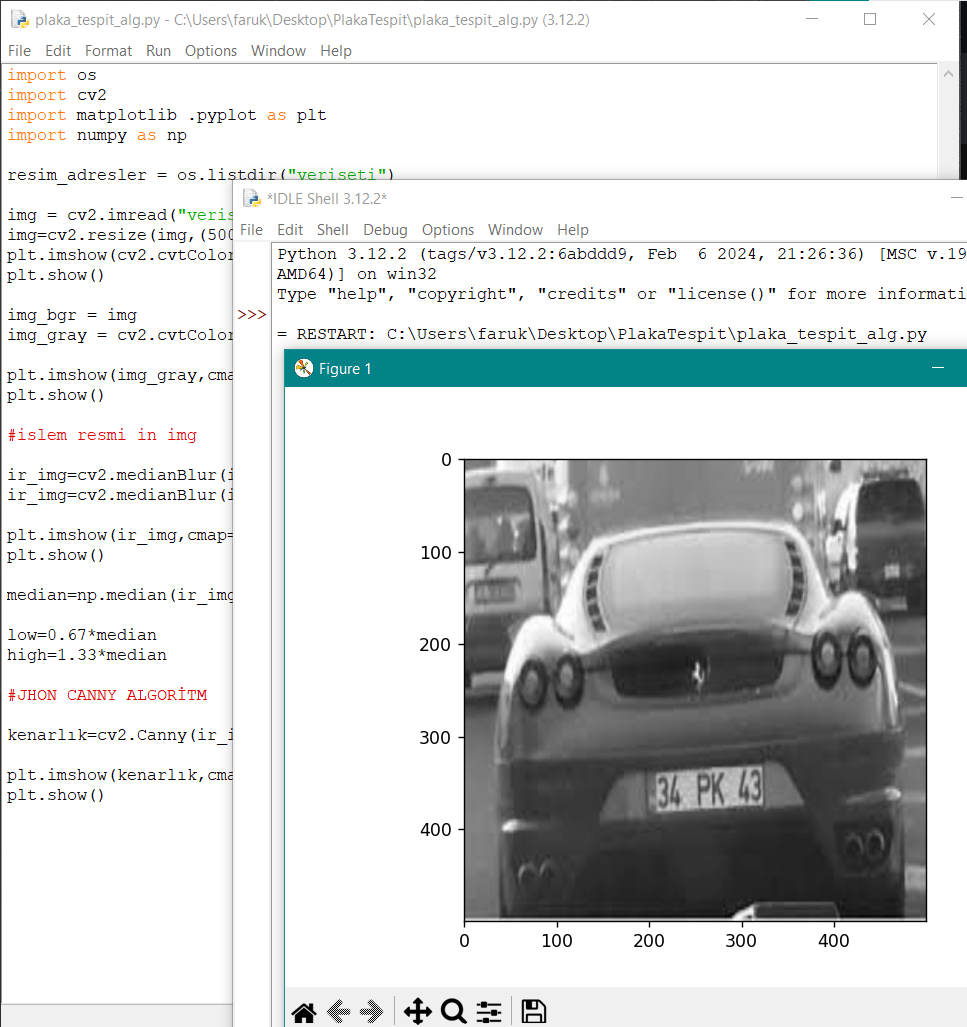
\includegraphics[	
			width=7cm,
			height=7cm,
			keepaspectratio,]{RenkGriCevirme.png}
			\caption{a)}
		\end{minipage}
		\hfill
		\begin{minipage}{0.45\textwidth}
			\centering
			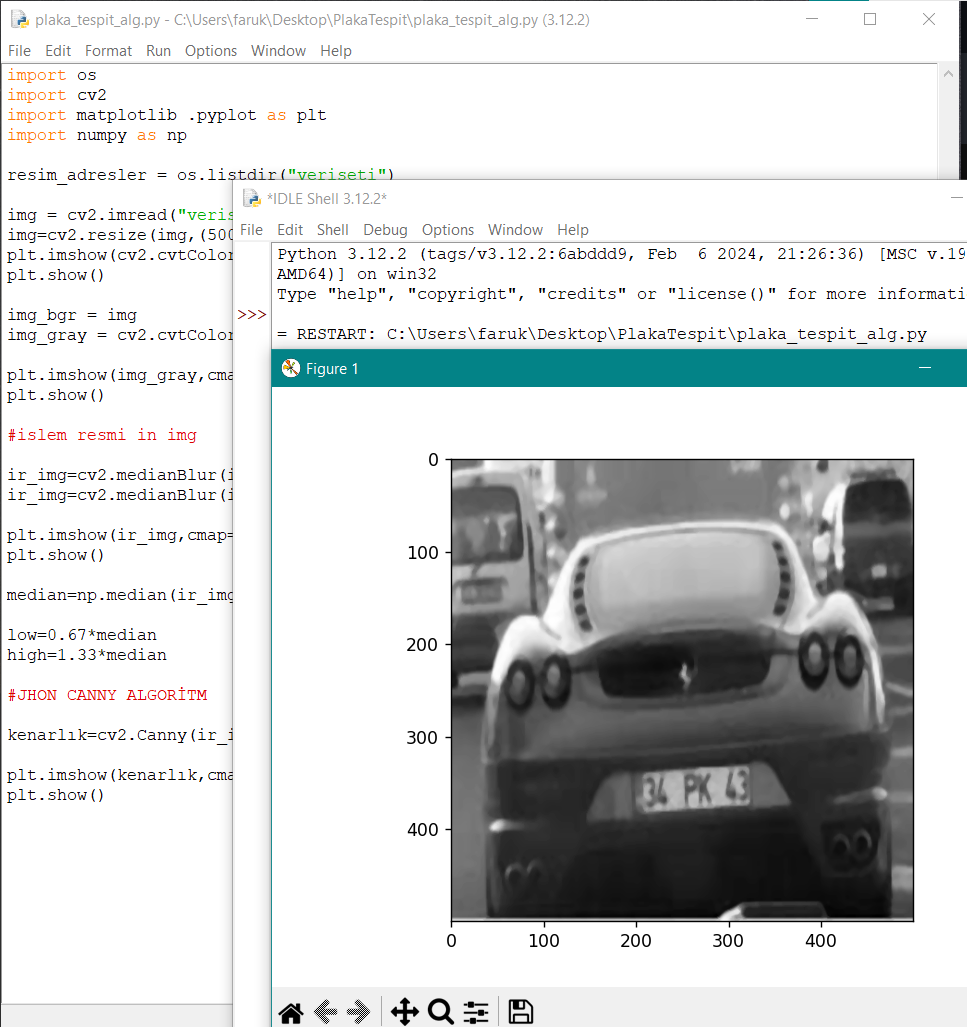
\includegraphics[	
			width=7cm,
			height=7cm,
			keepaspectratio,]{MedyanBulanıklaştırma.png}
			\caption{b)}
		\end{minipage}
		\newline
		\newline
		{a) Gri Formata Çevrilmiş Resim}
		{b) Medyan Bulanıklaştırma }
	\end{figure}
	\newpage
 	Jhon Canny Algoritması kullanılarak kenarların algılanması sağlandı ve kenarlıkların algılanmasının ardından ayrıştırma ve eşikleme işlemleri yapılarak plaka karakterlerinin daha iyi seçilmesi sağlanmaya çalışıldı.
	
	\begin{figure}[htbp]
		\centering
		\begin{minipage}{0.45\textwidth}
			\centering
			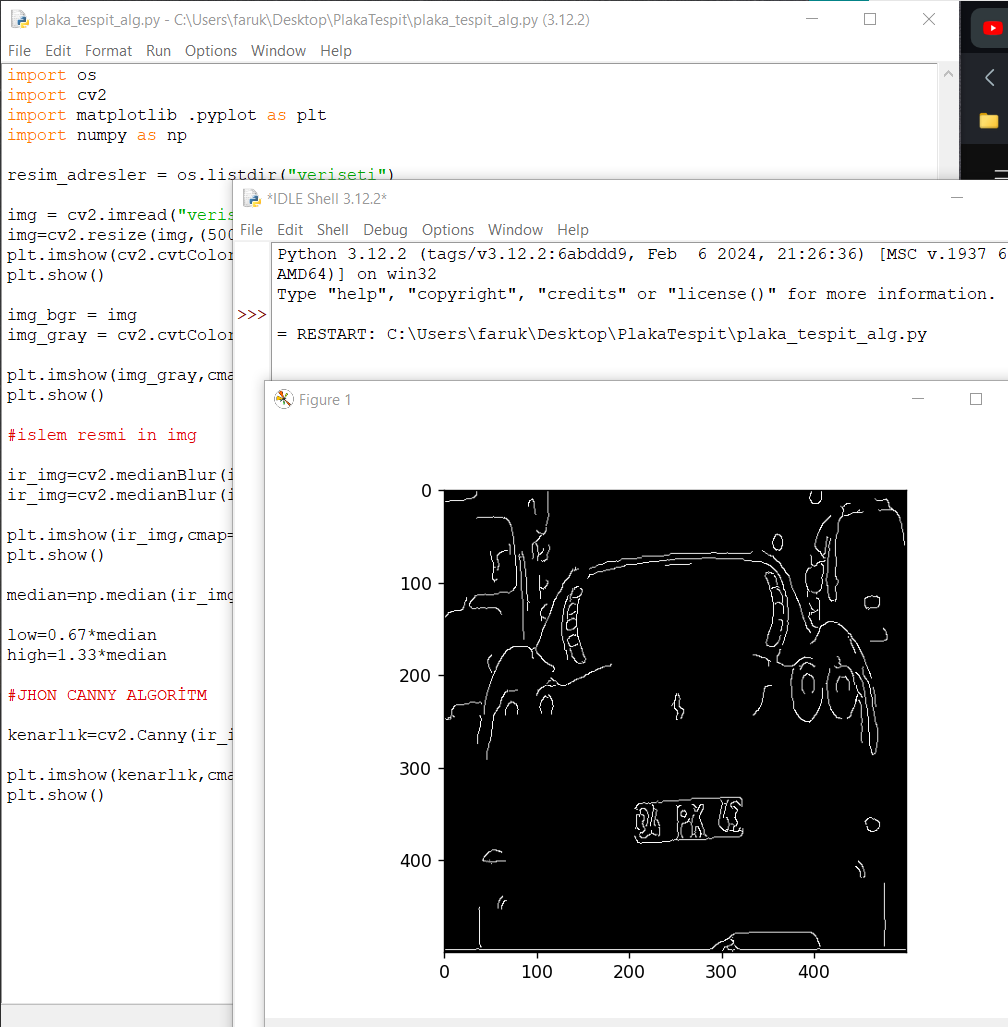
\includegraphics[
			width=7cm,
			height=7cm,
			keepaspectratio,]{CannyAlgoritm.png}
			\caption{a)}
		\end{minipage}
		\hfill
		\begin{minipage}{0.45\textwidth}
			\centering
			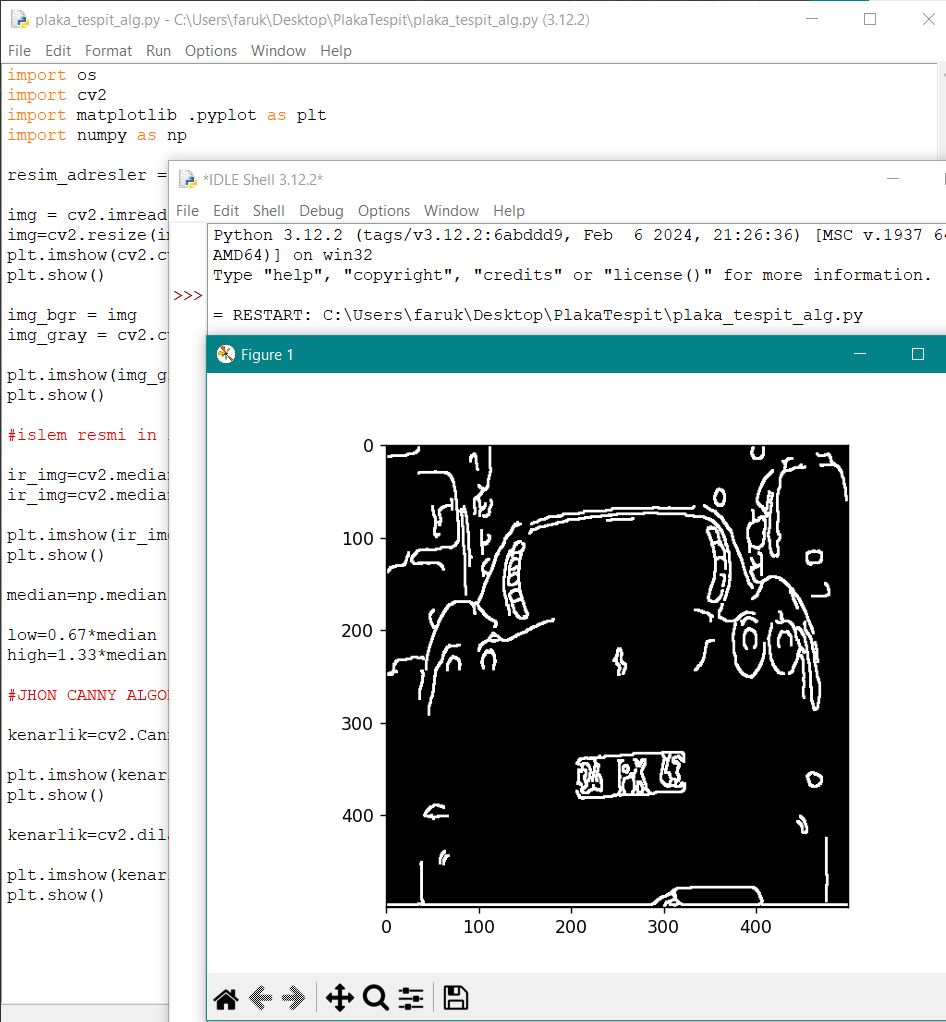
\includegraphics[
			width=7cm,
			height=7cm,
			keepaspectratio,]{GenisletilmeYapıldı.png}
			\caption{b)}
		\end{minipage}
		\newline
		\newline
		{a) Canny Algoritması Sonuc Çıktısı}
		{b) Genişletilme Yapıldıktan Sonra Görüntü }
	\end{figure}
	
	Projenin sonraki aşamasında ise, akıllı otopark sisteminin son bölümü için veri setinden alınmış plaka görüntülerinden, plakaları tanımak için bir makine öğrenimi modeli kullanıldı. Bu aşamada, yukarıda belirtilen önemli kütüphaneler import edilerek bir model dosyası (model.joblib) ve sınıf etiketleri belirlendi. Plaka görüntülerinin işlenmesi için gerekli işlevler ve işlem adımları tanımlanarak plakaların ayıklanması, plaka karakterlerinin tanınması ve tanınan karakterlerin plaka olarak düzenlenmesi gibi işlemler gerçekleştirildi. Kod içerisinde plaka tanıma işlemlerini gerçekleştiren bir fonksiyon olan "plakaTani" işlevi ile yapılmaya çalışıldı. Bu işlev, girdi olarak bir görüntü ve plakanın koordinatlarını alır ve plaka içindeki karakterleri tanımakla görevli fonksiyon işlevini görmektedir. Son olarak ise modelimizin denemeleri ve test aşamaları yapılarak hatalar ve ileride ne gibi düzeltmeler yapılacağı belirlendi.
	
	\begin{figure}[htbp]
	\centering
	\begin{minipage}{0.45\textwidth}
		\centering
		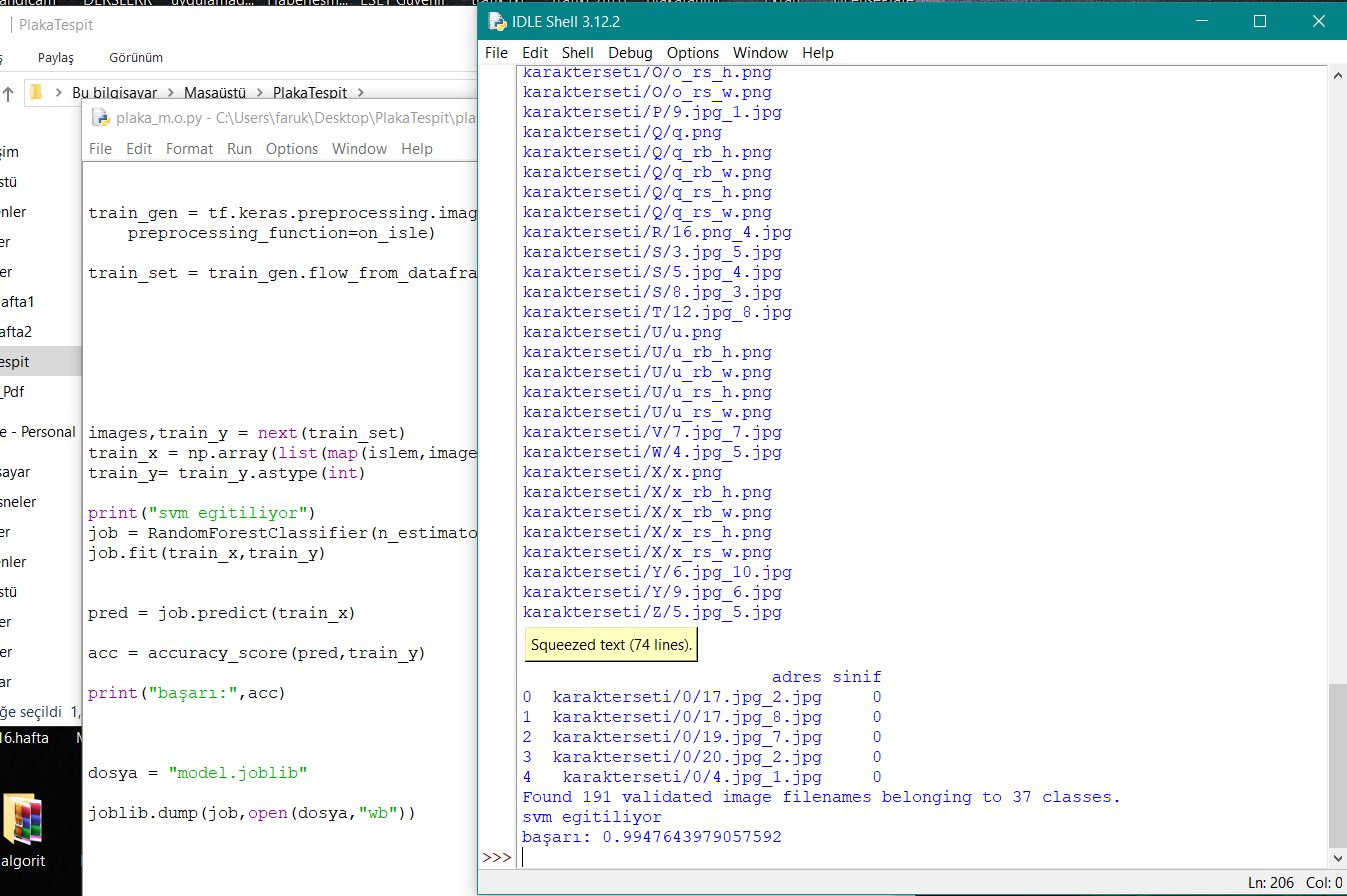
\includegraphics[	
		width=7cm,
		height=7cm,
		keepaspectratio,]{basari.png}
		\caption{a)}
	\end{minipage}
	\hfill
	\begin{minipage}{0.45\textwidth}
		\centering
		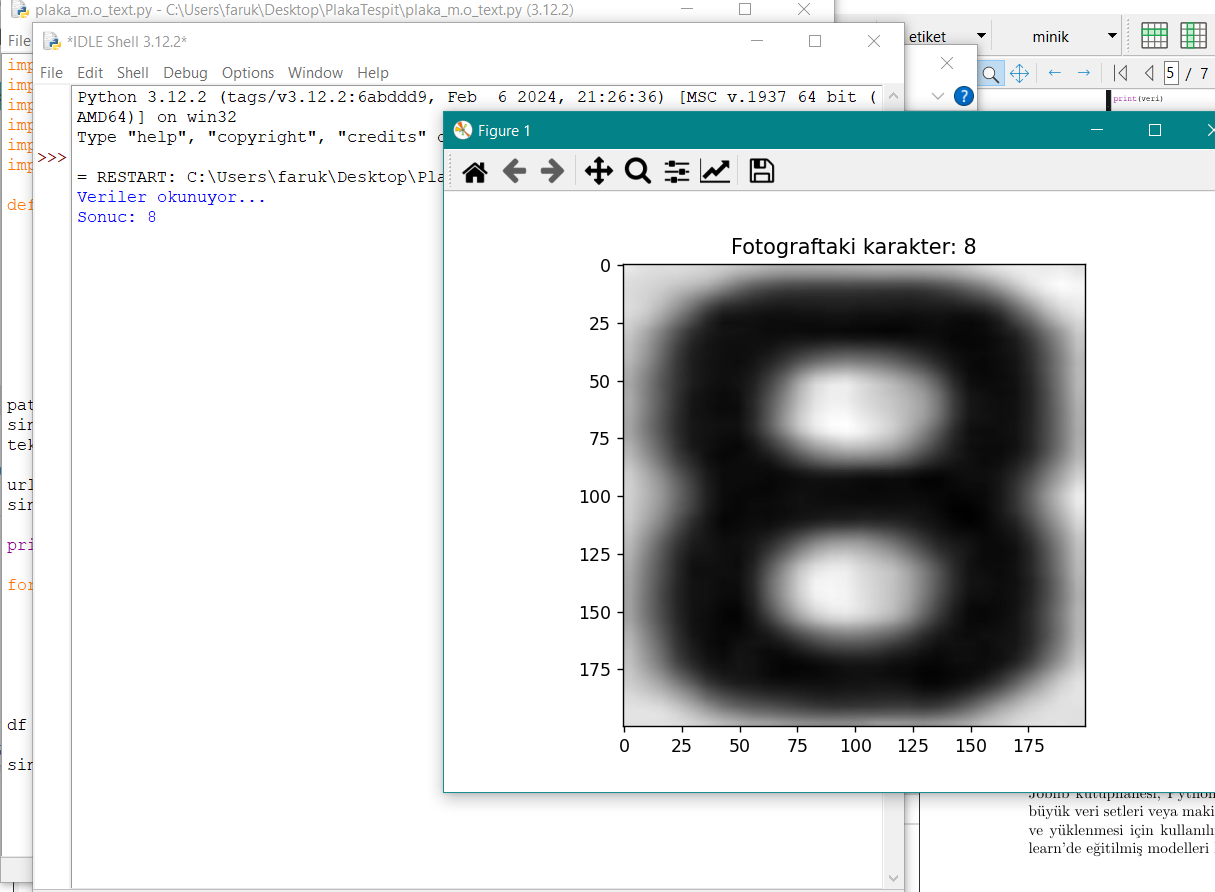
\includegraphics[	
		width=7cm,
		height=7cm,
		keepaspectratio,]{test.png}
		\caption{b)}
	\end{minipage}
\end{figure}
\begin{figure}[!htbp] %[h]
	\centering
	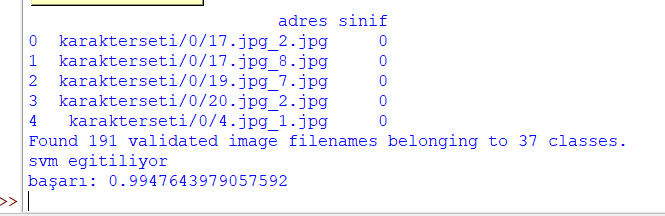
\includegraphics[
	width=11cm,
	height=11cm,
	keepaspectratio,
	]{basari2.png}
	\caption{c)} 
	{a) Makine Öğreniminin Sağlanması}
	{b) Test Verilerinin Denenmesi}
	{c) Başarı Oranının Çıktısı}
\end{figure}	
\newpage
	\subsection{İkinci Proje İçin Yapılanlar}
	Projenin ikinci aşamasında, yoğun bir bilgisayarla görme ve veri işleme çalışması gerçekleştirildi. Ana odak noktası, bir video dosyasındaki nesnelerin tespit edilmesi ve takip edilmesi üzerineydi. İlk önce resim incelenmek üzere ekran yansıtma gerçekleştirildi. Koda işaretlemeler yapılabilmesi için gerekli kod satırları yazıldı ve hatalı işaretleme durumu için silme işlemi kodu entegre edildi. İşaretlemeler yapılarak hem pickle hem de csv dosyasına kaydedildi.
	\begin{figure}[!htbp] %[h]
		\centering
		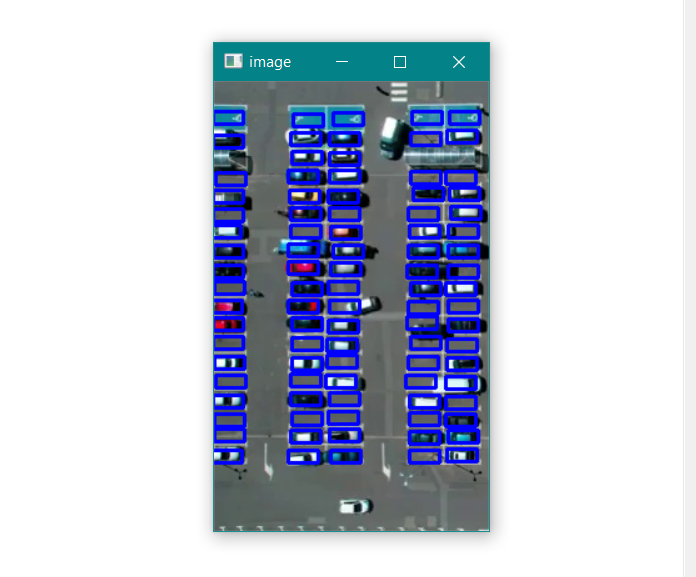
\includegraphics[
		width=8cm,
		height=8cm,
		keepaspectratio,
		]{opencvv.png}
		\caption{Otopark Alanlarının İşaretlenmesi}
	\end{figure}
	\\
	 Daha sonra video dosyası üzerinde nesne tespiti ve analizi yapmak ve doluluk boşluk durumunu öğrenmek için yeni dosya açılarak opencv kütüphanesi kullanılarak görüntü işleme teknikleri uygulandı; gri tonlamalı görüntüler elde etmek için renk dönüşümleri, median bulanıklığı ve adaptif eşikleme gibi yöntemler kullanıldı. 
	 
\begin{figure}[htbp]
	\centering
	\begin{minipage}{0.45\textwidth}
		\centering
		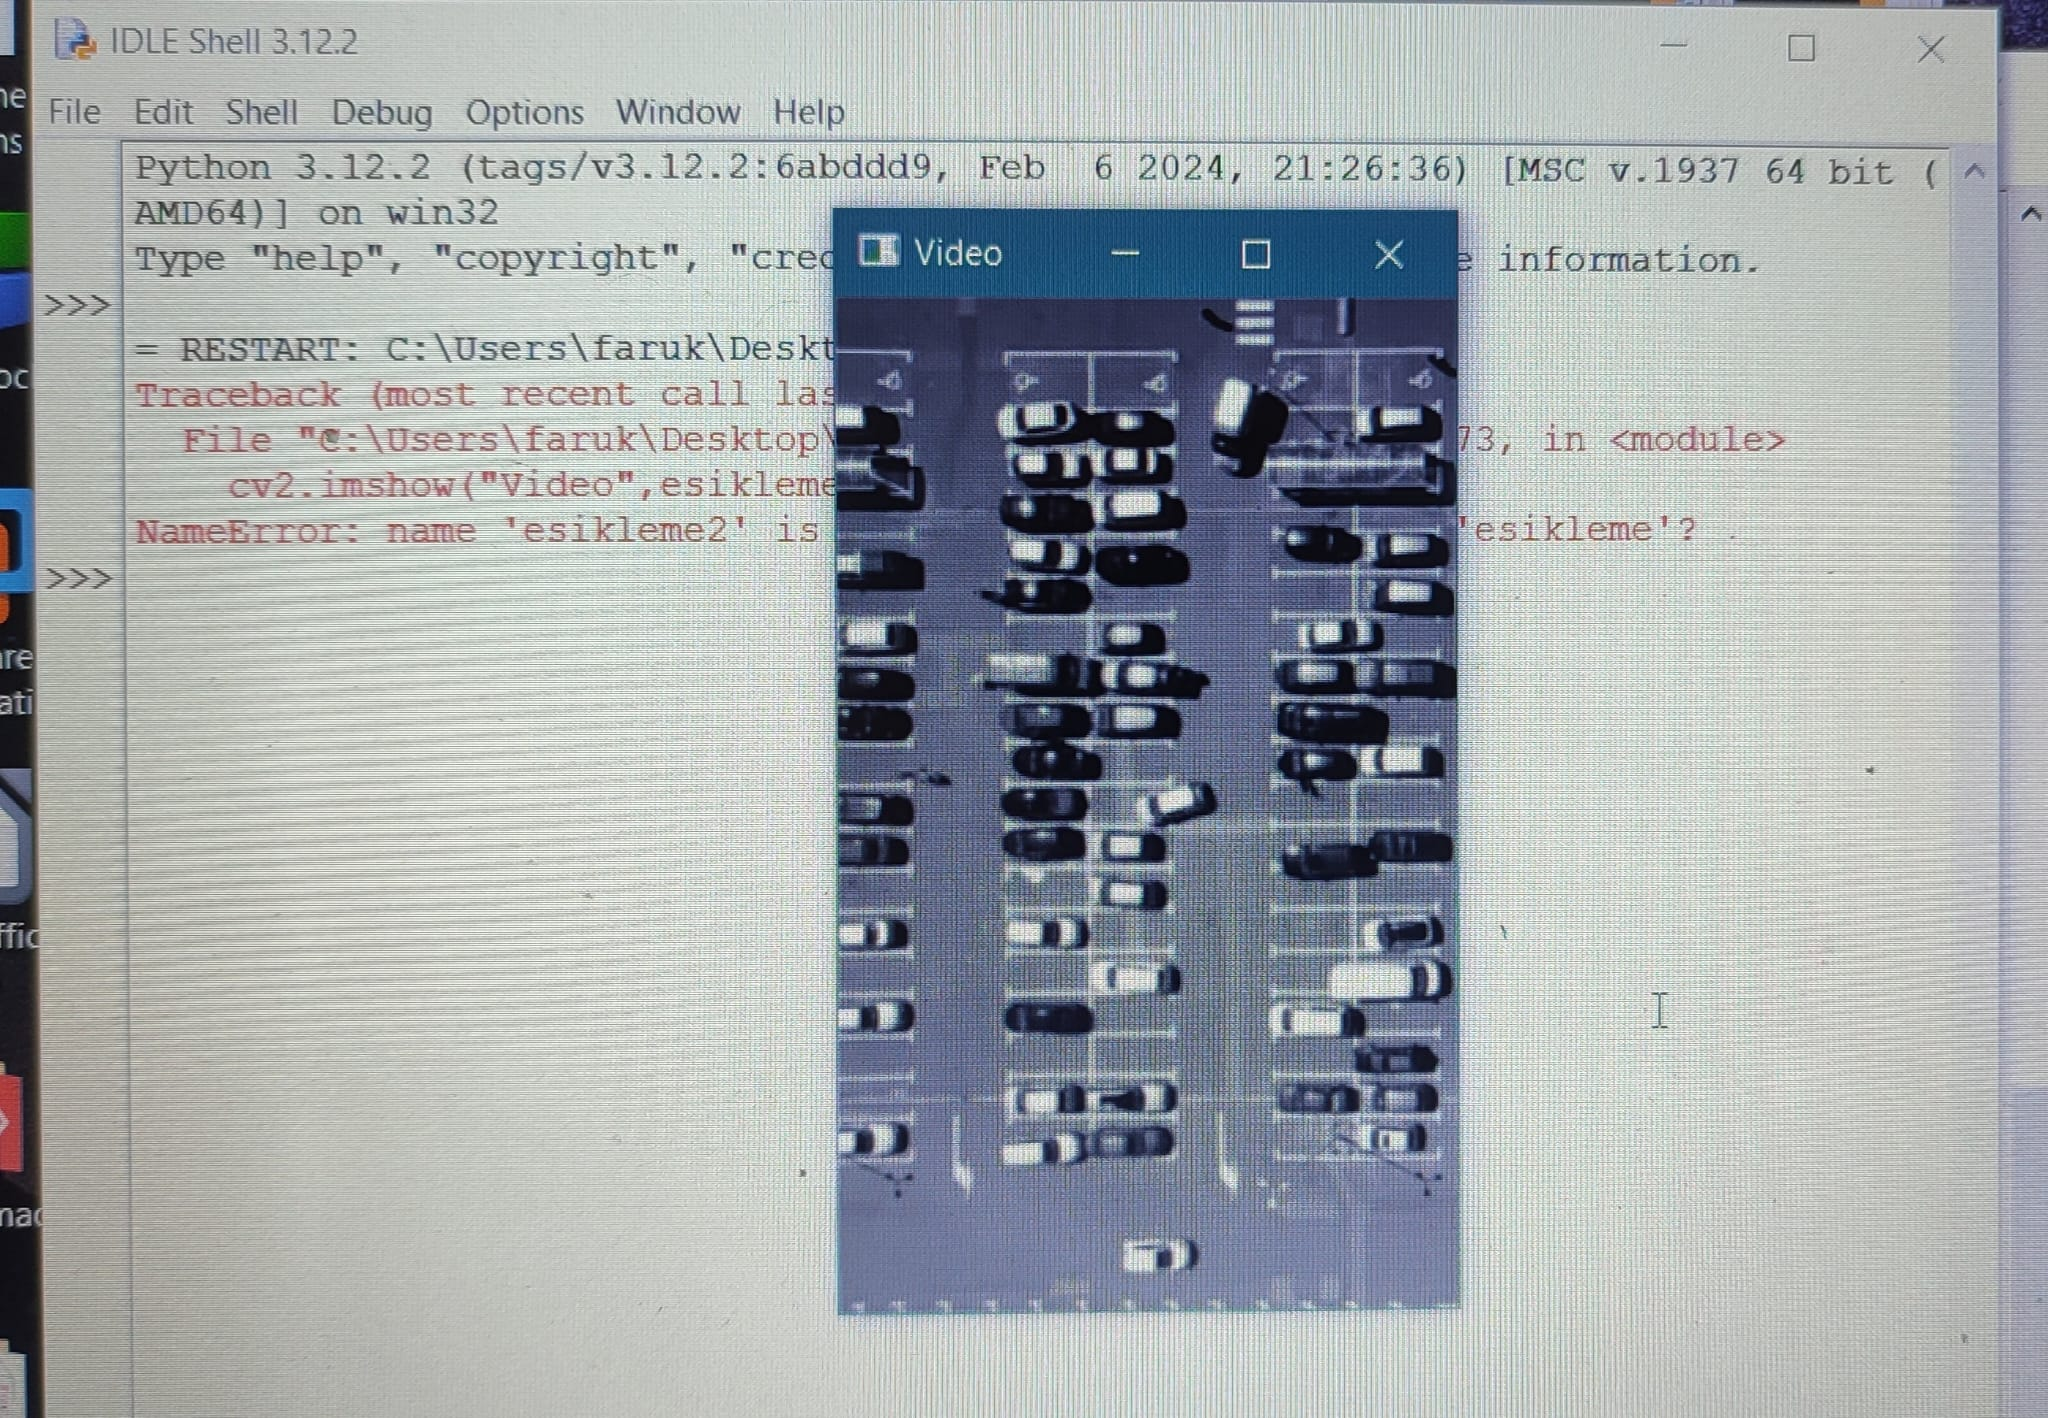
\includegraphics[	
		width=7cm,
		height=7cm,
		keepaspectratio,]{griformat.jpg}
		\caption{a)}
	\end{minipage}
	\hfill
	\begin{minipage}{0.45\textwidth}
		\centering
		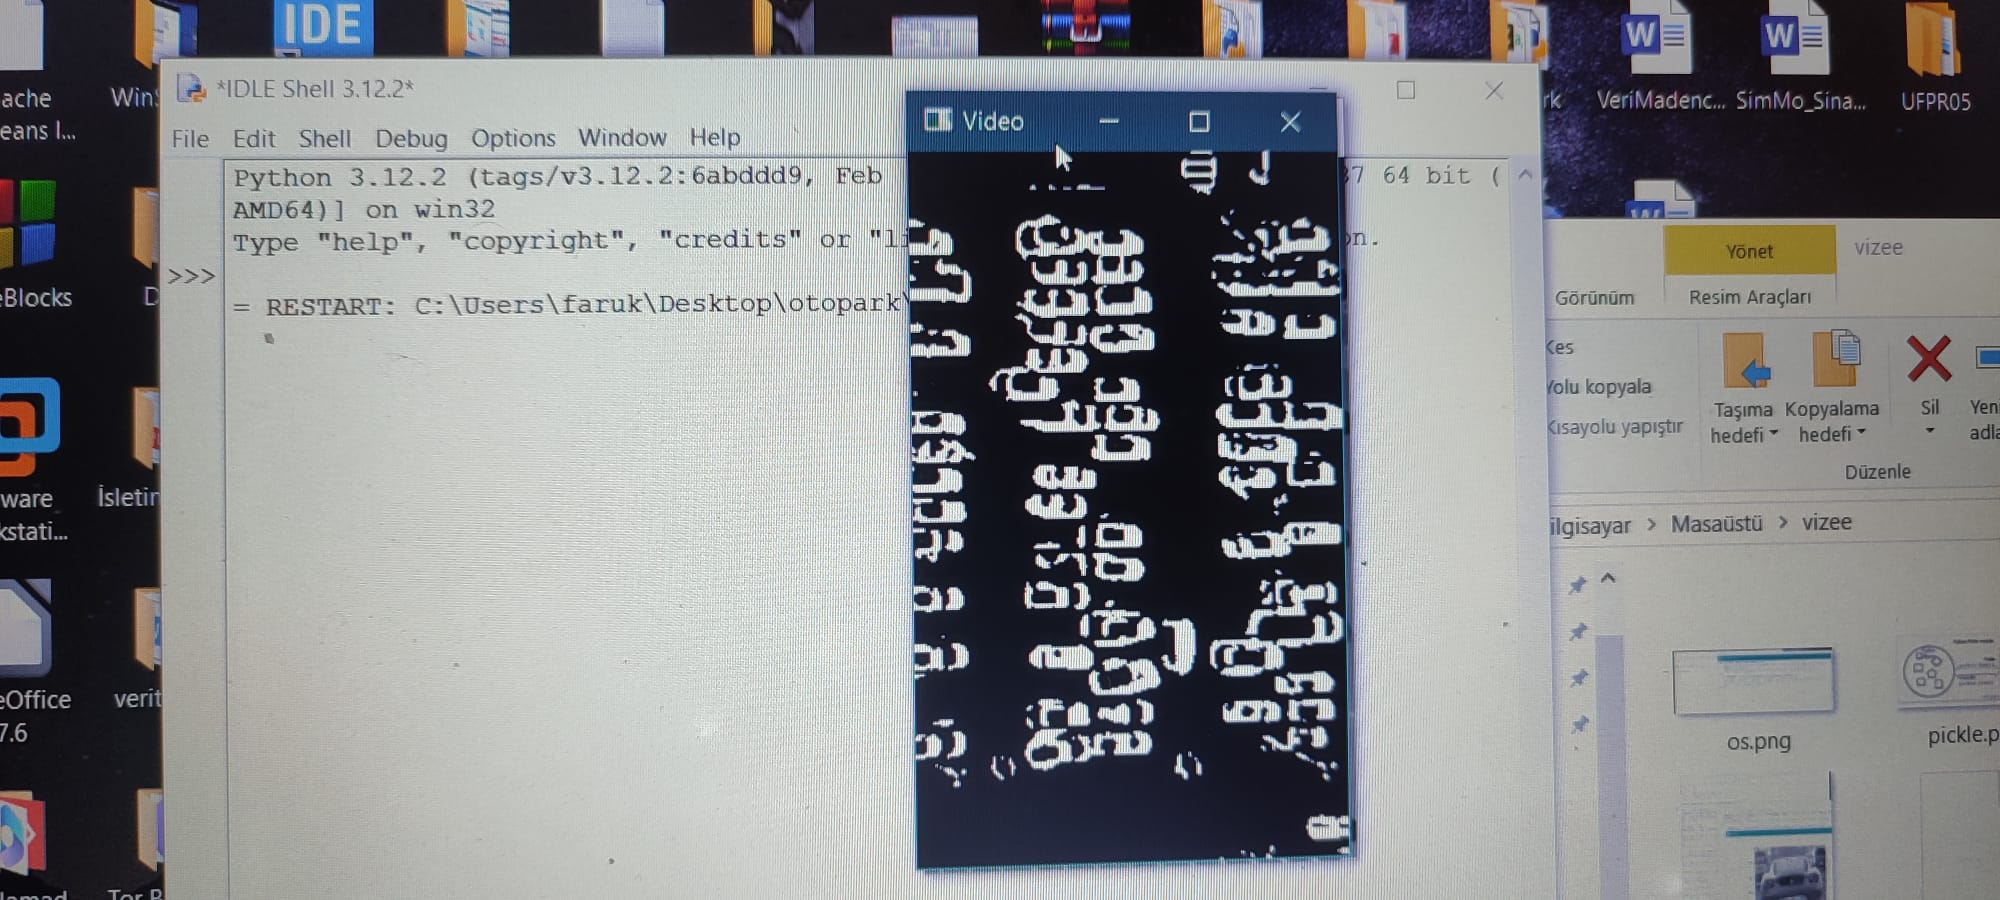
\includegraphics[	
		width=7cm,
		height=7cm,
		keepaspectratio,]{esikleme.jpg}
		\caption{b)}
	\end{minipage}
	\newline
	\newline
	{a) Resmin Gri Formata Dönüştürülmüş Hali}
    {b) Resmin Eşikleme Yapıldıktan Sonraki Hali }
	 
\end{figure}
\newpage
	Ardından, nesneler tespit edildi ve bu nesnelerin etrafına dikdörtgenler çizilerek görselleştirildi. Ayrıca, kullanıcı etkileşimli bir arayüz üzerinden nesne tespiti için referans noktaların belirlenmesini sağlayan bir sistem geliştirildi. Son olarak ise model test aşamasına sokularak gerekli bilgiler toplandı ve hataların neler olduğu bulundu. Bu bilgilerden yararlanılarak projenin nasıl ilerlenmesi gerektiği hakkında çıkarımlarda bulunuldu.
	
	\begin{figure}[!htbp] %[h]
		\centering
		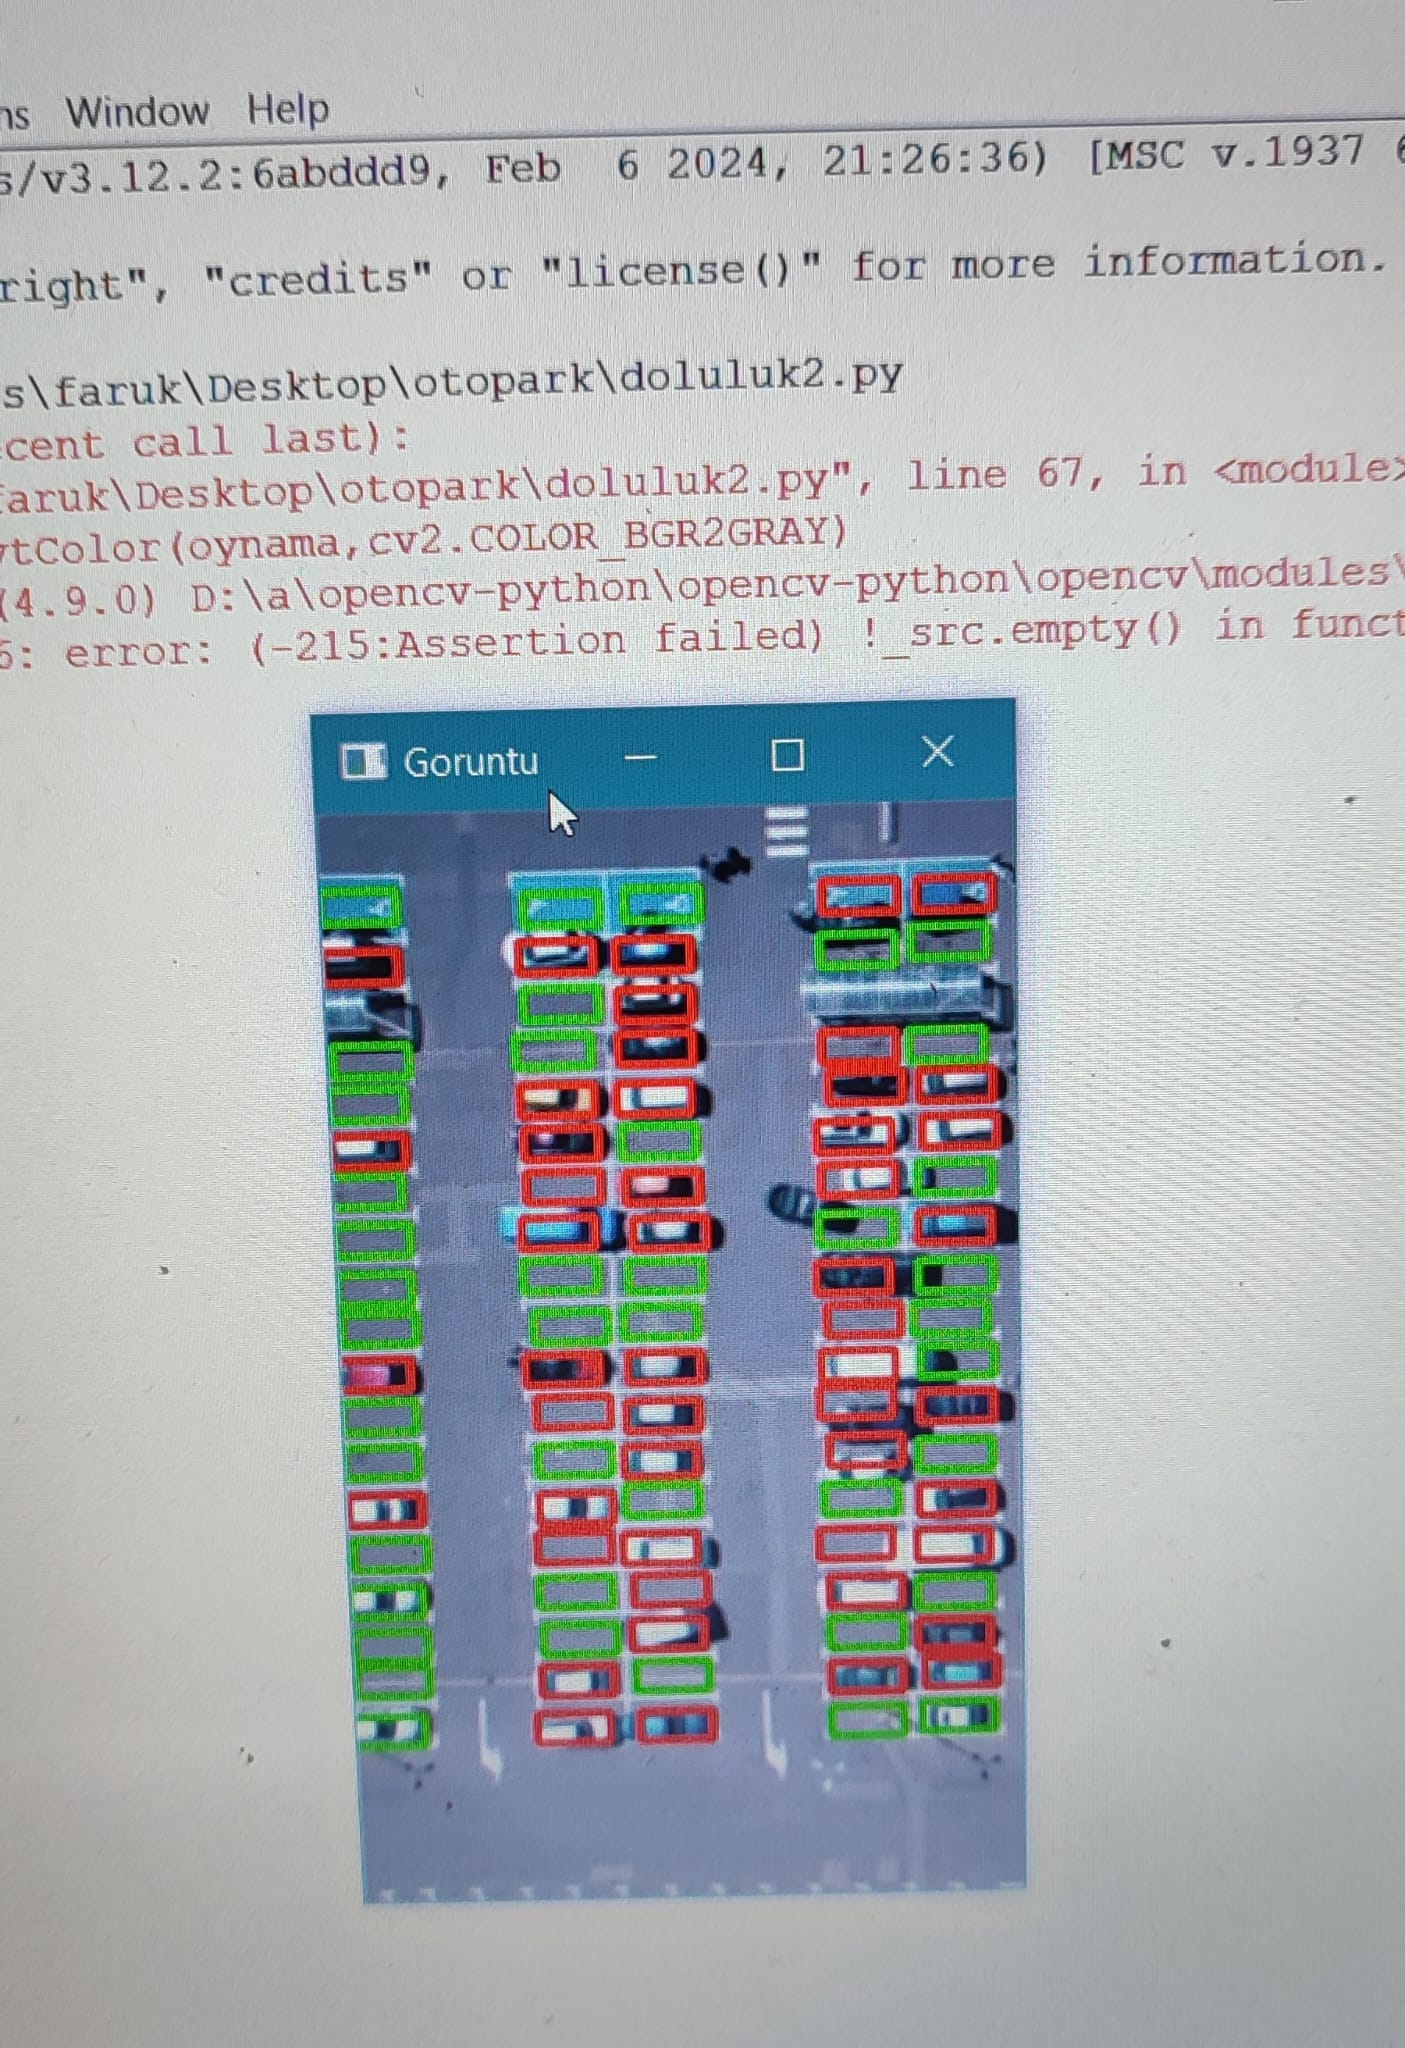
\includegraphics[
		width=8cm,
		height=8cm,
		keepaspectratio,
		]{sonmodel.jpg}
		\caption{Kurgulanan Modelin Çıktısı}
	\end{figure}
	\subsection{Bulgular ve Tartışma}
			\subsubsection{İşaretlenen Dataların Kayması}
			Bu hatada önceki kodda işaretlediğim dikdörtgenler belli konumdaydı. Mause ile basıldığında, noktayı ortalayarak dikdörtgen çiziliyordu. Fakat ikinci kodda, mause ile basılan nokta köşe olarak kabul edilip dikdörtgen öyle oluşturuluyordu. Bu da dikdörtgenlerin kaymasına ve otopark yerlerinin yanlış işaretlenmesine neden oluyordu. Bu hata birinci koddan aynı dikdörtgen hesabı kodu alınarak düzeltildi.
			
			\begin{figure}[!htbp] %[h]
				\centering
				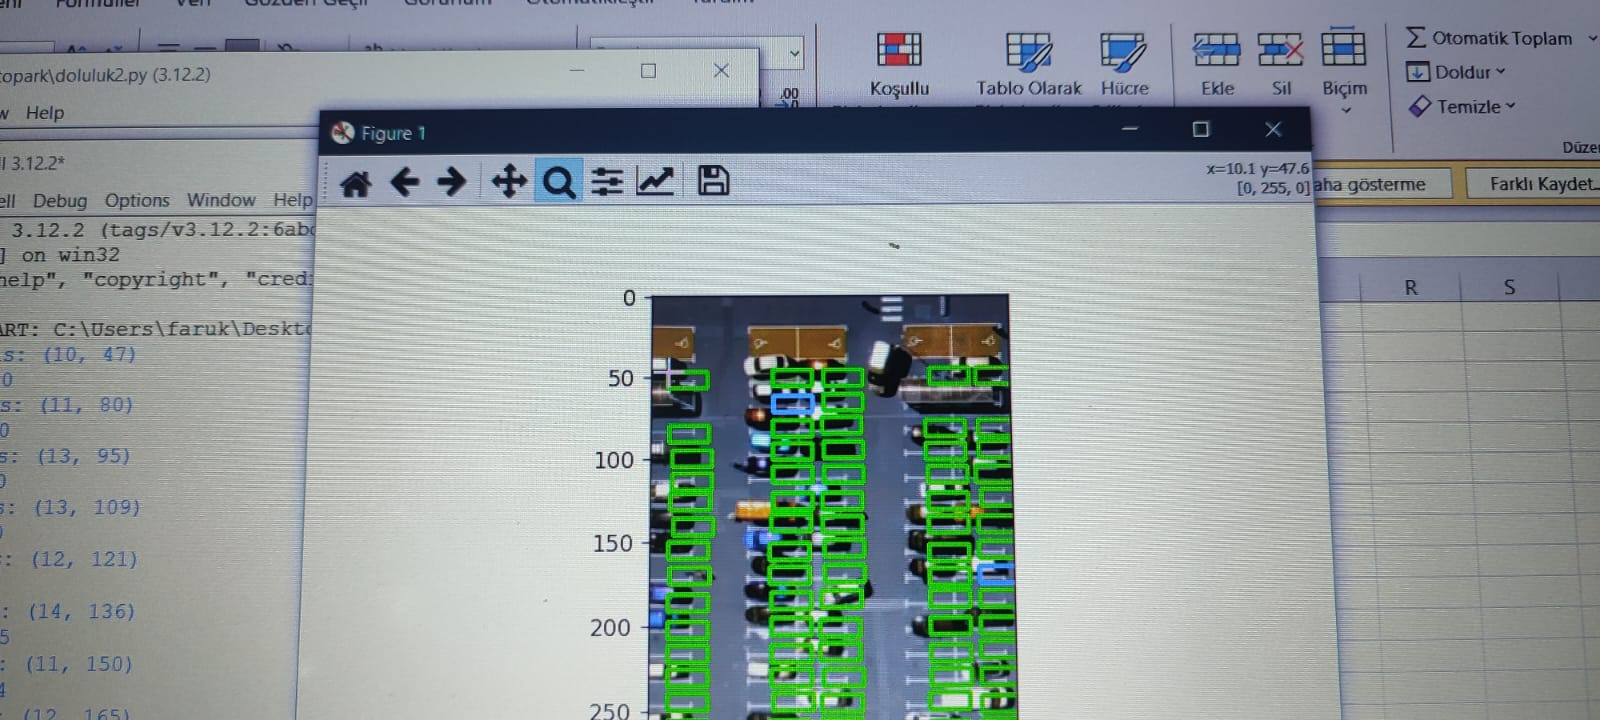
\includegraphics[
				width=11cm,
				height=11cm,
				keepaspectratio,
				]{hata1.jpg}
				\caption{Dataların hatalı bir şekilde kayması} 
			\end{figure}
			\newpage
			\subsubsection{Yanlış Gösterimler}
			Modelin büyük hatalarından birisi, yanlış gösterimdir. Makine öğrenimine sokulmadığından dolayı, oluşturulan model doluluk şeklini yoğunluğa göre belirlendi. Yani renk pikselleri 100'den fazla ise orada araba var ve otopark yeri dolu demektedir fakat bu, gölge çöktüğünde ya da aşırı güneş vurduğunda yanlış sonuçlara neden olmaktadır. Ayriyeten de insanlar geçtikçe de ani tepki vererek çok kısa süreliğine kırmızı yanmasına ve yanlış bilgiler oluşmasına neden olmuştur. Hala düzeltilme aşamasındadır. 
			\begin{figure}[!htbp] %[h]
				\centering
				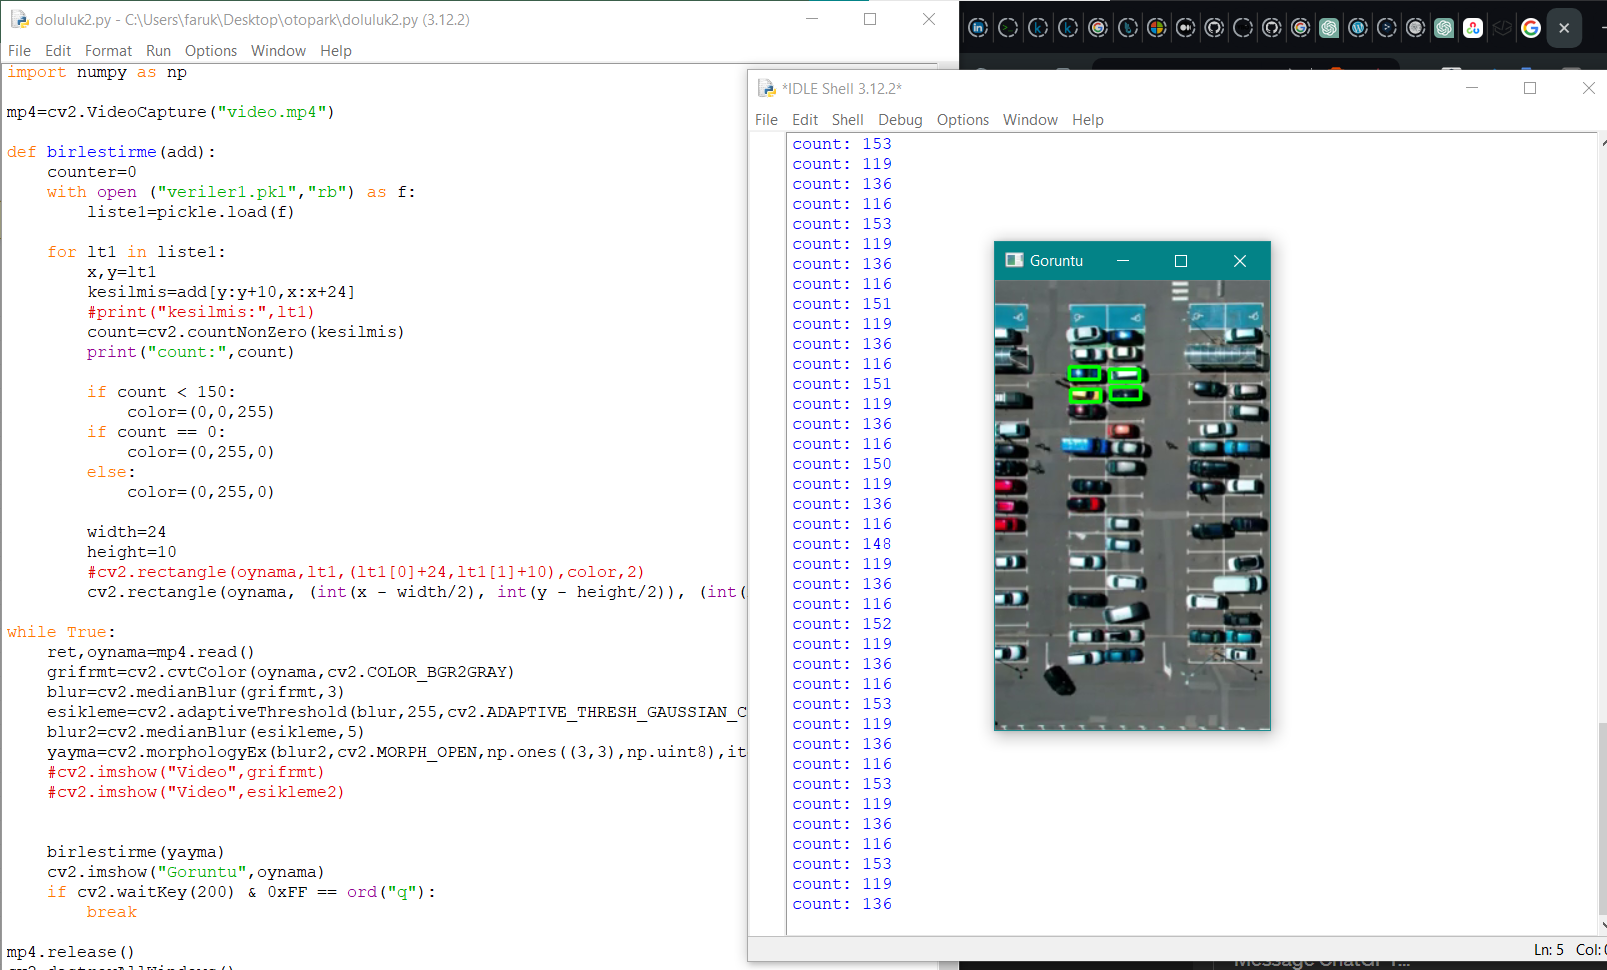
\includegraphics[
				width=9cm,
				height=9cm,
				keepaspectratio,
				]{hata2.png}
				\caption{Dataların hatalı bir şekilde kayması} 
			\end{figure}

	\subsection{Veriseti Bilgilendirme}
	Yapılan projelerden sonra konu hakkında bilgiler elde edilmiştir. Bundan sonra makine öğrenimi sürecine geçmek için hazırlıklar yapılmaktadır. İlk önce makine öğrenimi için dataset araştırıp bulunmuştur. 11gb olan datasette 3 farklı mekan için karlı,yağışlı ve güneşli gibi hava durumları olaylarında çekilmiş fotoğraflar vardır. Belli tarih ve günlerde çekilen fotoğraflarda, otoparkın dolu ve boş olduğu zamanlarda çekilen fotoğraflar sayesinde taglemeler yapılarak veriseti oluşturulmuştur. Boş otopark yerleri için 0 değeri verilmiş ve dolu otopark yeri için ise 1 değeri verilmiştir. Veri boyutu fazla olduğundan dolayı net bir şekilde ne kadar veri taglendiği bilinmemektedir.
	\begin{figure}[!htbp] %[h]
		\centering
		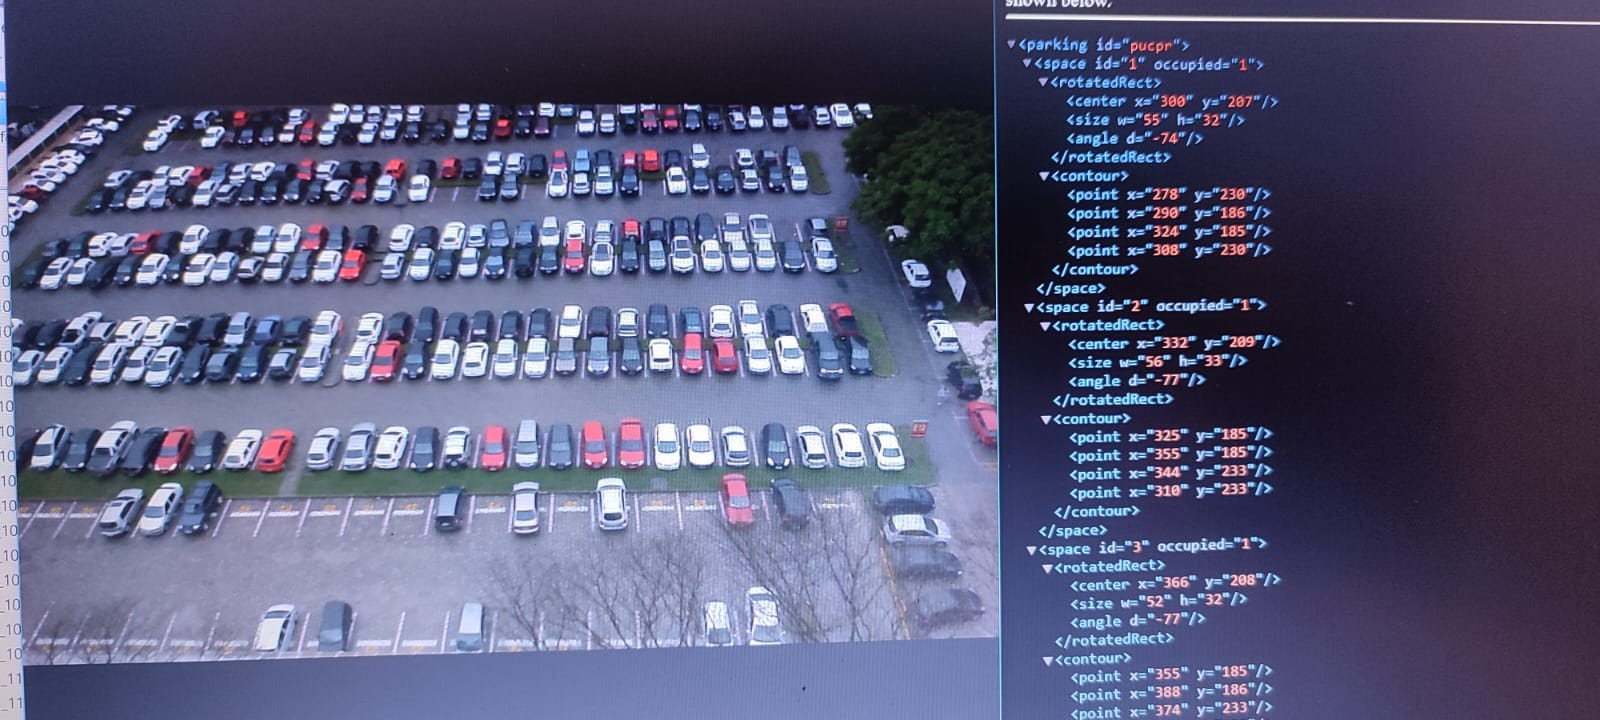
\includegraphics[
		width=11cm,
		height=11cm,
		keepaspectratio,
		]{dataset.jpg}
		\caption{Kullanılacak Dataset} 
	\end{figure}
	\newpage
	\subsection{Şuan Öğrenilmeye Çalışılan Kütüphaneler}
	Bu bölümde Projenin ilerleyişinde kullanılan ve öğrenerek kullanmam gereken kütüphaneler anlatılacaktır.
	\subsubsection{Opencv Kütüphanesi(CV2)}
	
	OpenCV (Open Source Computer Vision Library), bilgisayar görüşü ve görüntü işleme alanlarında yaygın olarak kullanılan açık kaynaklı bir kütüphanedir. Bu kütüphane, gerçek zamanlı görüntü işleme, nesne tanıma, nesne izleme, yüz tanıma, video analizi gibi birçok görevi gerçekleştirmek için bir dizi işlev ve algoritma içerir.
	
	\begin{figure}[!htbp] %[h]
		\centering
		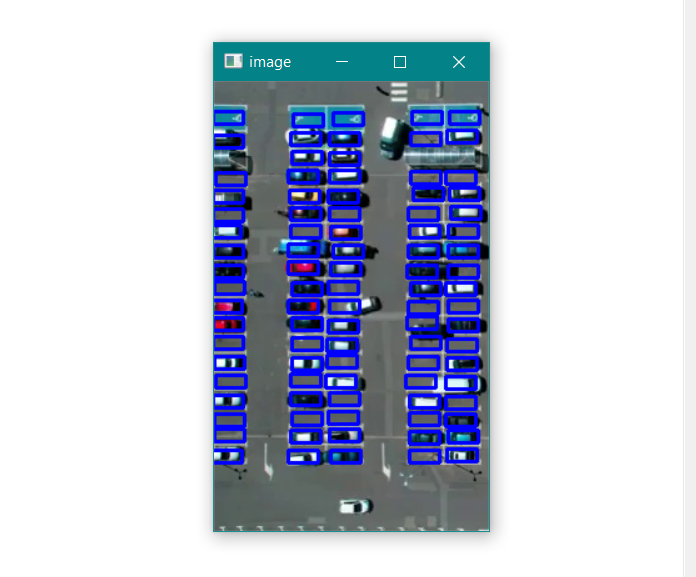
\includegraphics[
		width=9cm,
		height=9cm,
		keepaspectratio,
		]{opencvv.png}
		\caption{Opencv Kütüphanesi Kullanım Örneği}
	\end{figure}
	
	OpenCV'nin temel amacı, bilgisayarlı görüş ve görüntü işlemenin birçok yönünü desteklemek, araştırma yapmak ve gelişmiş uygulamalar oluşturmak için bir platform sağlamaktır. Yüz tanıma, nesne tanıma, nesne izleme, stereo görüş, hareket tespiti, görüntü segmentasyonu, derin öğrenme ve daha birçok görevi gerçekleştirebilen geniş bir işlev yelpazesi sunar.
	
	\subsubsection{Matplotlib Kütüphanesi(PLT)}
	Matplotlib, grafiklerin, histogramların, dağılım grafiklerinin, 3D grafiklerin ve daha birçok görsel öğenin oluşturulmasını sağlar. Ayrıca, interaktif grafikler oluşturmanızı da sağlayan çeşitli arayüzler ve grafik araçları sunar.\\
	Genellikle import matplotlib.pyplot as plt şeklinde kısaltılarak kullanılır. Bu, Matplotlib'in en popüler alt modülü olan pyplot modülünü içe aktarır ve kısayol olarak plt adını kullanır. Bu şekilde, Matplotlib'in çeşitli grafik oluşturma fonksiyonlarına daha kolay erişebilirsiniz.
	\begin{figure}[!htbp] %[h]
		\centering
		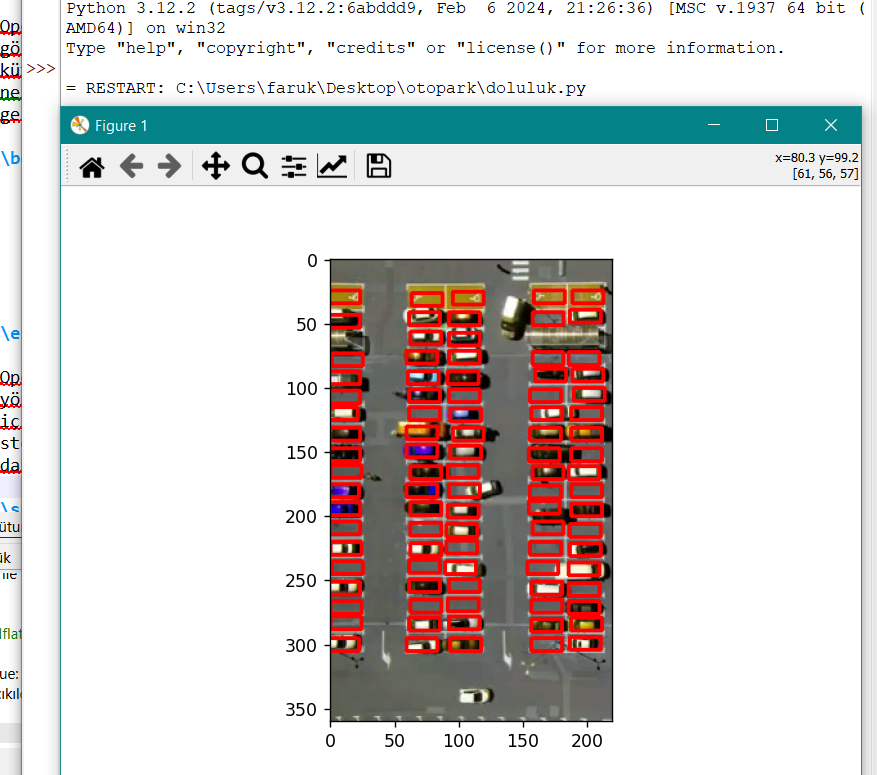
\includegraphics[
		width=7cm,
		height=7cm,
		keepaspectratio,
		]{plt.png}
		\caption{Matplotlib Kütüphanesi} 
	\end{figure}
	\subsection{Hangi Yapay Zeka Yöntemi}
	Bu projede, ilk olarak makine öğrenimi ile basit bir şekilde sistemin boş ve dolu yerlerinin algılanması sağlanacaktır. Bunu da daha önce yaptığımız plaka tanıma sistemine benzer şekilde öğrenilenler uygulanarak yapılacaktır. Ayriyeten son yapılan opencv ile otopark yer boş dolu sistemi geliştirilerek makine öğrenimine hazır hale getirilecek tüm otoparklarda çalışabilecek bir sistem tasarlanması için geliştirilecektir. Bu işlem bittikten sonra ise makine öğrenimi istenilen etkiyi ve doğruluğu vermez ise bu projeyi geliştirmek açısından derin öğrenme yöntemine başvurulacaktır. Bunu yapmamızın nedeni ise makine öğreniminin modelimizde yeterince düzgün çalışamamasından olacaktır. Bu işlem de bittikten sonra genel güncellemeler yapılarak akıllı otopark sistemimiz tam olarak hazır hale gelecektir.
	
	\subsection{Sonuç}
	Bu rapor, akıllı otopark sisteminin tasarımı ve geliştirilmesi üzerine yapılan bir çalışmanın sonuçlarını sunmaktadır. Geleneksel otopark sistemlerinin mevcut zorluklarını aşmak ve modern şehirlerdeki artan araç trafiği sorunlarına çözüm getirmek amacıyla, plaka tanıma teknolojisi ve görsel tanıma algoritmalarının kullanımıyla bir sistem tasarlanmıştır. Çalışmanın sonuçları, mevcut sistemlerin iyileştirilmesine dair önemli ipuçları sunmaktadır. Ancak, derin öğrenme ve makine öğrenimi gibi daha ileri seviye tekniklerin uygulanmasına henüz geçilmemiştir.
	\newpage
	\bibliographystyle{ieeetr}
	\bibliography{reference1.bib}
	\dots{}
	
\end{document}
